\subsection{Performance Evaluation}
\label{sec:evaluation}
%\textcolor{red}{Three machines connected in an isolated 1Gbps LAN,
%    build the experimental SSO environment.
%The CPUs are Intel Core i7-4770 3.4 GHz for the IdP,
%    Intel Core i7-4770S 3.1 GHz for the RP, and Intel Core i5-4210H 2.9 GHz for users.
%Each machine is configured with 8 GB RAM and
%    installs Windows 10 as the operating system.
%The user agent is Chrome v75.0.3770.100.}

%RP(不包括特定方案的SDK)大约需要230行JAVA代码
%OIDC(MITREid)的SDK需要大约20行的JAVA代码,需要额外添加一个HTML文件(包含大约20行JavaScript代码)
%UPPRESSO的SDK需要大约1100行代码,不需要添加额外的HTML文件
%OIDC和UPPRESSO的SDK只需要RP提供两个网络接口(网址),然后在对应的网络接口中引用对应的API(每个接口对应一个API,分别命名为tokenRequestGenerate和userAccountAchieve),其他的处理流程均由SDK完成
%SPRESSO由于结构与OIDC完全不同,所以使用了SPRESSO提供的RP的开源代码
%For better evaluation, we build one RP for both UPPRESSO and MITREid Connect which is also implemented  based on Spring Boot framework, as well as the identity token transmission from user to RP in MITREid Connect is implemented by JavaScript running in RP's web page. The IdP in MITREid Connect is achieved from github \cite{MITREid}. However, the SPRESSO system is downloaded from \cite{spressome} containing IdP, RP and FWD.

\noindent {\bf Experiment setting.} We compared \usso\ comprehensively with MITREid Connect and SPRESSO.
MITREid Connect supports the implicit flow of OIDC,
 while SPRESSO follows a similar approach to forward the identity token from a user to the RP.
 SPRESSO encrypts the RP's domain in identity tokens and keeps the symmetric key known only to the RP and the user. Both systems employ RSA-2048 and SHA-256 for token generation.
SPRESSO implements all entities by JavaScript based on node.js, while MITREid Connect provides Java implementations of IdP and RP SDKs.
Therefore, for \usso\ and MITREid Connect, we implemented RPs based on Spring Boot by integrating the respective SDKs. In all three schemes, the RPs provide the same function of obtaining the user's account from verified identity tokens.

The IdP and RP servers were deployed on Alibaba Cloud Elastic Compute Service, each running Windows 10 with 8 vCPUs and 32 GB memory. The forwarder of SPRESSO ran Ubuntu 20.04.4 with 16 vCPUs and 16 GB memory, also on Alibaba Cloud.

We conducted experiments in two scenarios: (\emph{a}) a browser, Chrome 104.0.5112.81, ran on a virtual machine with 8 vCPUs and 32 GB memory on Alibaba Cloud, and (\emph{b}) a browser running locally on a PC with Core i7-8700 CPU and 32 GB memory, remotely accessed the servers.
In the cloud scenario, all entities were deployed in the same virtual private cloud and connected to one vSwitch, which minimized the impact of network delays. In both scenarios, the IdP server never directly communicated with the RPs.

\noindent {\bf Comparisons.} We split the login flow into three phases for detailed comparisons: (1)
{\em identity-token requesting} (Steps 1 and 2 of the \usso\ protocol), to construct an identity-token request and send it to the IdP server; (2) {\em identity-token generation} (Step 3), to generate an identity token at the IdP server, while the user authentication and the user-attribute authorization are excluded; and (3) {\em identity-token acceptance} (Step 4), where the RP receives, verifies, and parses the identity token.


We compared the average time required for an SSO login in three schemes based on 1,000 measurements. As shown in Figure \ref{fig:evaluation},
MITREid Connect, \usso, and SPRESSO require (\emph{a}) 63 ms, 179 ms, and 190 ms, respectively when all entities were deployed on Alibaba Cloud,
 or (\emph{b}) 312 ms, 471 ms, and 510 ms, respectively when the user browser ran locally to visit the cloud servers.

Regarding identity-token requesting, %the user browser loads the RP's webpage and starts the login request.
the RP of MITREid Connect immediately constructs an identity-token request. %MITREid Connect only needs 10 ms but UPPRESSO requires 271 ms.
In contrast, \usso\ incurs an extra overhead in opening a new browser window and downloading scripts.\footnote{This overhead may be reduced %by silently conducting these operations when the user visits the RP website, or
by implementing a user agent with browser extensions.
% but users need to install the extension before visiting RPs.
We implemented such a browser extension while keeping the IdP and RPs unmodified. Our experiments showed a reduction of about 90 ms in the virtual private cloud setting and 260 ms when accessed remotely.}
The RP in SPRESSO needs to obtain information about the IdP % 's public key %(SPRESSO allows a user to assign any IdPs before login without initial registrations)
and encrypt its domain using an ephemeral key, resulting in additional overheads.

\begin{figure}[tb]
  \centering
	\subfigure[In a virtual private cloud]{
  		\begin{minipage}[b]{0.455\textwidth}
			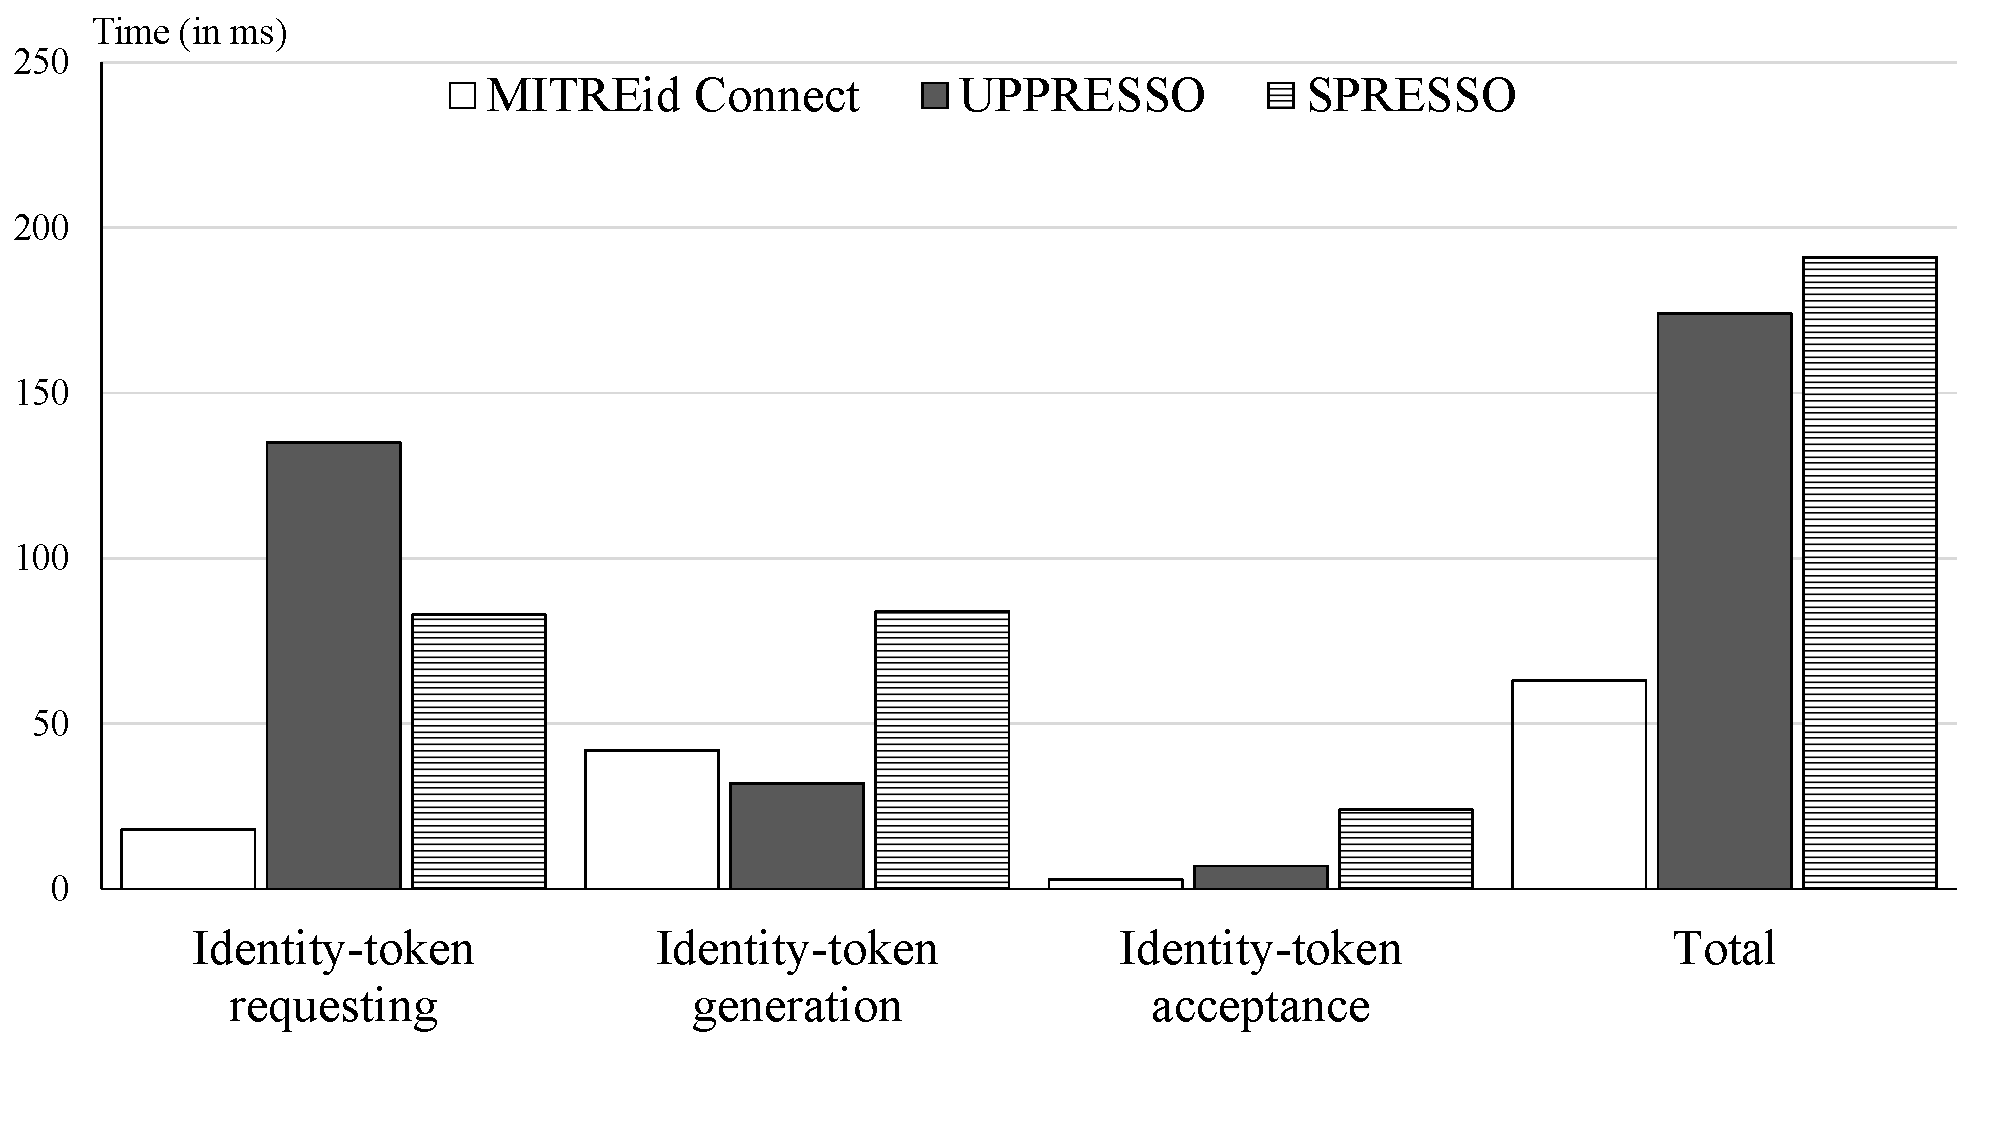
\includegraphics[width=0.973\linewidth]{fig/evaluation-lan.pdf}
		\end{minipage}}
	\subfigure[With a remotely-visiting browser]{
  		\begin{minipage}[b]{0.455\textwidth}
			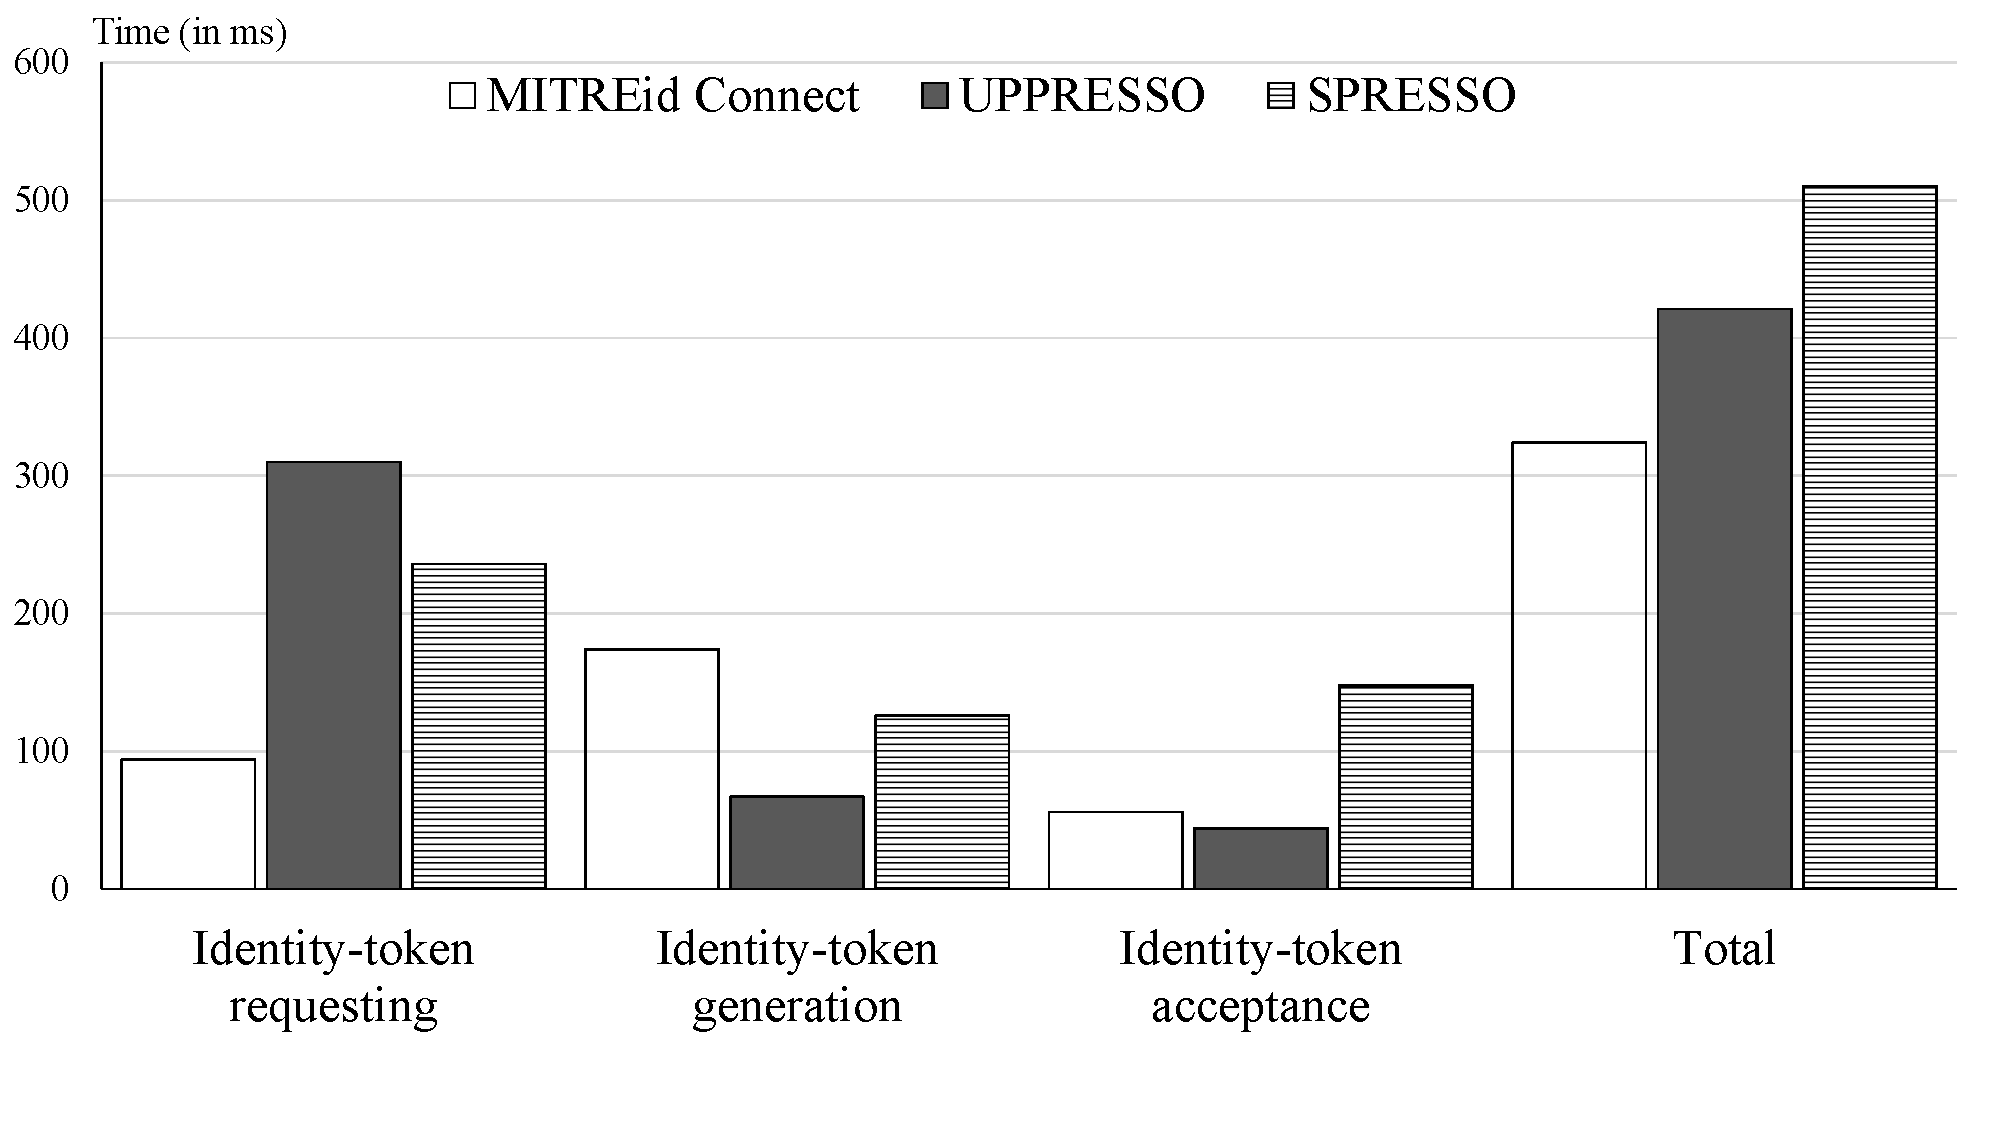
\includegraphics[width=0.973\linewidth]{fig/evaluation-internet.pdf}
		\end{minipage}}
  \caption{The time cost of SSO login}
  \label{fig:evaluation}
\end{figure}

Compared with the two schemes, \usso\ requires less time for identity token generation since it retrieves the token from the IdP without any additional processing. In contrast,
MITREid Connect requires more time as the user is required to download a script from the RP to process the token retrieved from the IdP, which is carried with a URL following the fragment identifier \verb+#+ instead of \verb+?+ due to security considerations \cite{de2014oauth}. SPRESSO takes slightly more time to generate an identity token as it implements the IdP using node.js and uses a JavaScript cryptographic library less efficient than the Java library used by the other two schemes.

%transmission & extraction
In the identity-token acceptance phase, MITREid Connect and \usso\ take similar amounts of time to send an identity token to the RP and verify it.
In contrast, SPRESSO takes the longest time due to its complex process at the user agent.
After receiving the identity tokens from the IdP, the browser needs to download JavaScript code from the trusted forwarder server, decrypt the RP endpoint, and then send the identity tokens to this endpoint.

